\section{Intermediate values: \addbs{tkzTabVal}}
This macro places a value on an arrow of the line of variations. It must be used just after the command \tkzcname{tkzTabVar} that defines the line of variations where the intermediate values go. A value can only be placed on an interval where the function is \tkzname{monotonic}. The macro also shows a new (intermediate) value of the variable in the first row.

\subsection{Definition of \addbs{tkzTabVal}}

\begin{NewMacroBox}{tkzTabVal}{\oarg{local options}\{Begin\}\{End\}\{Position\}\{Value\}\{Image\}}

\begin{tabular}{lllc}
\toprule
\texttt{arguments}   & \texttt{default}    & \texttt{definition}                        \\
\midrule
\IargName{tkzTabVal}{Begin}     & |no default|  & rank of the start of the arrow       \\
\IargName{tkzTabVal}{End}       & |no default|  & rank of the end of the arrow     \\
\IargName{tkzTabVal}{Position}  & |no default|  & decimal number between $0$ and $1$      \\
\IargName{tkzTabVal}{Value}& |no default|  & value of the variable, if needed \\
\IargName{tkzTabVal}{Image}     & |no default|  & value of the function, if needed     \\
\bottomrule
\end{tabular}

\medskip
\noindent\emph{Some comments: the first thing is to choose the arrow on which the image is placed. \tkzname{Begin} and \tkzname{End} are the ranks of the values at the ends of the arrow. \tkzname{Value} and \tkzname{Image} are the values to place. \tkzname{Position} is a number between $0$ and $1$: an abscissa on the arrow, with \tkzname{Begin} as origin and \tkzname{End} as end.}

\medskip
\begin{tabular}{lllc}
\toprule
\texttt{options}   & \texttt{default}    & \texttt{definition}                                      \\
\midrule
\IoptName{tkzTabVal}{draw}    & |false|   & draws an arrow from the value to its image     \\
\IoptName{tkzTabVal}{remember}& |lastval|& gives a name to the node of the image                   \\
\bottomrule
\end{tabular}

\medskip
\noindent\emph{For an arrow from the value to its image, use the option \tkzname{draw}. To refer later to the point where the image is, use the option \tkzname{remember}.}
\end{NewMacroBox}

\subsubsection{Adding intermediate values}

The first example shows remarkable values of the function $\ln$. The function is monotonic between the values of rank $1$ ($0$) and $2$ ($+\infty$), so the first two arguments are $1$ and $2$. The coefficients used for \tkzname{Position} are \tkzname{decimal} numbers, here $0.33$ and $0.66$. The values of the variable were not in the first row, so they are given as arguments.

\begin{tkzexample}[code only]
    \tkzTabVal{1}{2}{0.33}{1}{0}
    \tkzTabVal{1}{2}{0.66}{\E}{1}
\end{tkzexample}

\begin{tkzexample}[vbox, small]
\begin{tikzpicture}
\tkzTabInit[lgt=3,espcl=10] {$x$    /1, Sign\\ of $\dfrac{1}{x}$  /1.5,%
                       Variations\\ of $\ln$   /2} {$0$ , $+\infty$}%
    \tkzTabLine{d,+,}%
    \tkzTabVar[color=red]{ D- /  $-\infty$, + /  $+\infty$ }
    \tkzTabVal{1}{2}{0.33}{1}{0}
    \tkzTabVal{1}{2}{0.66}{\E}{1}
\end{tikzpicture}
\end{tkzexample}

\subsubsection{Intermediate values with a function that is not monotonic}

The macro can only be used on an interval where the function is monotonic. Here there are three values,
\mbox{$0$, $\E$ and $+\infty$}. The function is monotonic between the first two, that is between the values of rank $1$ and $2$, and between the last two, of rank $2$ and $3$.

\begin{tkzexample}[vbox,small]
\begin{tikzpicture}
  \tkzTabInit[espcl=6]{$x$ / 1 , $f'(x)$ / 1, $f(x)$ / 2}
                      {$0$, $\E$ , $+\infty$}%
  \tkzTabLine{d,+,0,-,}%
  \tkzTabVar{D- / $-\infty$, + / $\E$, - / $0$  }%
  \tkzTabVal[draw]{1}{2}{0.6}{$1$}{$\dfrac{1}{\E}$}%
  \tkzTabVal[draw]{2}{3}{0.4}{$\E^2$}{$1$}%
\end{tikzpicture}
\end{tkzexample}

\subsubsection{Intermediate values with a plateau}

Do not stop at the second value. The function is monotonic but has a plateau. The symbol \tkzname{R} prevents an arrow from stopping at $\sqrt\E$, so the arrow goes from the value of rank $1$ to the value of rank $3$. The code is:
\begin{tkzexample}[code only]
  \tkzTabVal[draw]{1}{3}{0.6}{\E}{$\dfrac{-1}{\E}$}
\end{tkzexample}

\begin{tkzexample}[vbox,small]
\begin{tikzpicture}
 \tkzTabInit[espcl=6]{$x$/1,$f'(x)$/1, $f(x)$/2}
                     {$0$,$\sqrt\E$,$+\infty$}%
 \tkzTabLine{d,+,0,+,}%
 \tkzTabVar{D-  / $-\infty$,R  /     ,+  / $0$  }
 \tkzTabVal[draw]{1}{3}{0.4}{$1$}{$-\E$}
\end{tikzpicture}
\end{tkzexample}


\subsubsection{Intermediate values and several lines of variations}
\Iopt{tkzTabVal}{draw}

The variations of $f$ and $f'$ are shown. For $f$, the value $1$ is not used, so we go from rank $1$ to rank $3$.

\begin{tkzexample}[vbox,small]
\begin{tikzpicture}
  \tkzTabInit[espcl=6]{$x$/1,$f''(x)$/1,$f'(x)$/3,$f(x)$/3}
  {$0$,$1$,$+\infty$}%
  \tkzTabLine{d,+,0,-, }%
  \tkzTabVar{-/ $-\infty$ ,+/ ,-/ $-\infty$ }
  \tkzTabVal[draw]{1}{2}{0.3}{$0.3$}{$-2$}
  \tkzTabVal[draw]{2}{3}{0.6}{$4$}{$-1$}
  \tkzTabVar{+/ $+\infty$,R ,-/ $-1$}
  \tkzTabVal[draw]{1}{3}{0.6}{$2$}{$0$}
\end{tikzpicture}
\end{tkzexample}

\subsection{Using the options}

\subsubsection{\texttt{\textcolor{red}{draw}}: an arrow to the added value}\Iopt{tkzTabVal}{draw}
The option was already used in the previous examples; here is another one.

\begin{tkzexample}[vbox,small]
\begin{tikzpicture}
 \tkzTabInit[lgt=3,espcl=10]{$x$                 /1,
                       Sign\\ of $\dfrac{1}{x}$ /2,
                       Variations\\ of $\ln$      /3}
                       {$0$           , $+\infty$  }%
 \tkzTabLine           {d,+           ,            }%
 \tkzTabVar[color=red]{D-/ $-\infty$ , +/$+\infty$}%
 \tkzTabVal[draw]{1}{2}{0.24}{\scriptsize $1-h$}{$<0$}%
 \tkzTabVal[draw]{1}{2}{0.3}{$1$}{$0$}%
 \tkzTabVal[draw]{1}{2}{0.36}{\scriptsize $1+h$}{$>0$}%
 \tkzTabVal[draw]{1}{2}{0.64}{$2.7$}{$<$}%
 \tkzTabVal[draw]{1}{2}{0.7}{$\E$}{$1$}%
 \tkzTabVal[draw]{1}{2}{0.76}{$2.8$}{$>$}%
\end{tikzpicture}
\end{tkzexample}


\subsubsection{\texttt{\textcolor{red}{remember}}: giving a name to a point or a node}
\Iopt{tkzTabVal}{remember}

This option is useful with \tkzcname{tkzTabImaFrom}, and the named nodes can also be used with any \TIKZ\ code.

\begin{tkzexample}[code only]
  \draw[opacity=0.4,fill=red!20]  (vb) circle(3ex);
  \draw[opacity=0.4,fill=blue!20]  (vc) circle(3ex);
\end{tkzexample}


\begin{tkzexample}[,small]
  \begin{tikzpicture}
  \tkzTabInit[lgt=3,espcl=6]{ $x$/1,/1,/3,/3 }%
             {  $a$    , $d$    ,$e$}
  \tkzTabLine{  z,+    ,z,-     ,z  }
  \tkzTabVar  {-/\va  ,+/\vd   , -/  \ve}

  \tkzTabVal[draw,remember=vb]{1}{2}{0.333}{$b$}{$0$}
  \tkzTabVal[draw,remember=vc]{1}{2}{0.666}{$c$}{$1$}

  \tkzTabVar{-/\va  ,R/   , +/  \ve}

  \tkzTabVal[draw]{1}{3}{0.5}{}{$0$}

  \draw[opacity=0.4,fill=red!20]  (vb) circle(3ex);
  \draw[opacity=0.4,fill=blue!20]  (vc) circle(3ex);
  \end{tikzpicture}
\end{tkzexample}

\medskip
Note that $b$ and $c$ are intermediate values: the table was defined with $a$, $d$ and $e$.
\endinput